% !TeX spellcheck = da_DK
\subsection{Filter}
\subsubsection{Teori og design}
%Efter signalet er blevet forstærket skal det filtreres, så alle de uønskede signaler kan dæmpes. Der benyttes kun et lavpasfilter, da det ønskede signal ifølge litteraturen kan ligge i frekvensområdet $0-10$Hz, som beskrevet i afsnit \ref{FilterAfs} på side \pageref{FilterAfs}. Jævnfør pilotforsøget i afsnit \ref{Sec:PilotforsoegKort}, side \pageref{Sec:PilotforsoegKort} blev der målt et signal i frekvensområdet $0-25$Hz og det frekvensområdet sættes derfor til $0-25$Hz, for at filtrere uønskede signaler fra. 
Filtre kan udarbejdes både i aktiv og passiv form. Hvis signalet ligger i frekvensområdet under $1$MHz anbefales det at benytte aktive filtre. Aktive filtre benytter operationforstærkere, kondensatorer og modstande, hvor passive filtre benytter kondensatorer, modstande og spoler. \cite{Carter2013} Der findes flere forskellige typer filtre, heriblandt Butterworth-, Tschebyschev- og Besselfilter. Butterworthfilteret giver maksimal fladhed i pasbåndet og stopbåndet. Tschebyschevfilteret giver den hurtigste overgang fra pasbåndet til stopbåndet. Besselfilteret giver en lineær faserespons, hvilket vil sige at fasen er lineær med frekvensen.\fxnote{Til os: Fasen angiver hvor godt et signals frekvensspektrum bliver gengivet}\fxnote{skal vi have et billede ind af de forskellige typer?} \cite{Carter2013} I dette projekt anvendes et Butterworthfilter, da der ønskes maksimal fladhed i pasbåndet og stopbåndet som nævnt i kravspecifikationerne for filtret. De forskellige typer filtre fremgår af nedestående figur \figref{fig:type_filtre}. \fxnote{kilde?}

\begin{figure}[H]
	\centering
	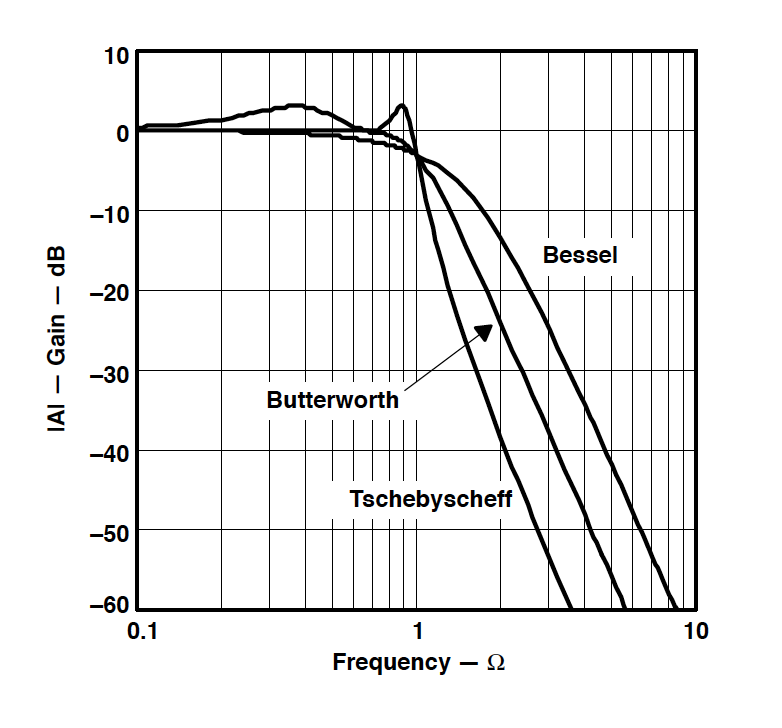
\includegraphics[scale=0.8]{figures/cProblemloesning/type_filtre.PNG}
	\caption{Figuren viser et bodeplot filter, hvor de fire karakteristika af et lavpasfilter er angivet}
	\label{fig:type_filtre}
\end{figure}

Der findes to forskellige måder hvorpå et filter kan designes: Sallen-Key topologien (SKT) og Multiple Feedback toppologien (MFT). SKT-metoden er den mest anvendte og tillader separate gain indstillinger samt inverterende og ikke-inverterende konfigurationer, hvorimod MFT-metoden benyttes i filter design med høj gain-nøjagtighed eller høj Q-værdi. I dette projekt benyttes en ikke-inverterende konfiguration grundet den høje indgangsimpedans i den ikke-inverterende terminal, hvorfor SKT-metoden er valgt. Herved forhindres loading af filtrets output. Loading defineres som effekten af, at et spændingsmålende instrument bruger strømmen i et kredsløb og kan være både ønsket og uønsket i et system. Der må eksempelvis gerne være loading, hvis det ønskes at tænde for en lampe eller en højtaler. Loading-effekten er derimod en uønsket effekt for dette projekts system, da der ønskes et lavt effektforbrug, hvilket giver en lang levetid. Loading reducerer den samlede strøm, som løber i kredsløbet, og trækker meget strøm fra batteriet. \\
Hvis der vælges en inverterende operationsforstærker i filterkonfiguration, falder den samlede resistans, og der kræves derfor mere strøm for at opretholde outputspændingsniveauet. Eftersom den ikke-inverterende forstærker i filteret har høj inputimpedans, hvilket vil sige, at modstanden i operationsforstærkeren har en høj værdi, vil filterets output ikke blive påvirket af loading. \cite{Webster2009,Carter2013,Karni2014}

Jævnfør kravspecifikationer af lavasfilteret i afsnit \ref{FilterAfs}, side \ref{FilterAfs} kræves det, at filteret har en minimumsdæmpning af stopbåndet $(min_{A})$ på $14$dB og der accepteres en maksimal dæmpning af pasbåndet $(max_{A})$ på $3$dB. Derudover skal lavpasfilteret have en knækfrekvens $(\omega _p)$ på $25$ Hz, samt en stopbåndsfrekvens $(\omega _s)$ på $45$ Hz. Af nedestående figur \figref{fig:lavpasfilter_generisk} fremgår en illustration af, hvad de forskellige parametre beskriver.

\begin{figure}[H]
	\centering
	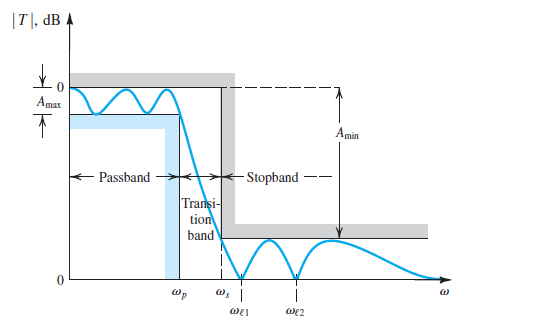
\includegraphics[scale=0.8]{figures/cProblemloesning/Lavpasfilter_generisk.PNG}
	\caption{Figuren viser et bodeplot filter, hvor de fire karakteristika af et lavpasfilter er angivet}
	\label{fig:Lavpasfilter_generisk}
\end{figure}

\noindent Med udgangspunkt i de enkelte parametre af lavpasfilteret kan den pågældende orden af filteret bestemmes vha. \eqref{lavpasfilter} for overføringsfunktionen:
\begin{equation} \label{eq:lavpasfilter}
A(\omega_s) = 10 \text{log} \cdot \left[1 + \epsilon^2 \cdot (\frac{\omega _s}{\omega _p})^{2N}\right] 
\end{equation}

\noindent I \eqref{eq:lavpasfilter} er filterets orden angivet af N. Når de resterende variabler kendes, kan lavpasfilterets orden udregnes. I formelen betegner $A(\omega _s)$ den minimale dæmpning der kræves af stopbåndet, hvor $\epsilon$ er udtrykt ved nedestående \eqref{epsilon}:
\begin{equation}\label{eq:epsilon}
\epsilon = \sqrt{10^{\frac{A_{max}{10}} - 1}}
\end{equation}

Nu kan lavpasfilterets orden bestemmes, jævnfør værdierne fra kravspecifikationerne fra afsnit \ref{FilterAfs}, side \pageref{FilterAfs} ved at indsætte disse værdier i \eqref{eq:lavpasfilter}. Udregningerne vil se ud som følgende:
\begin{equation}
\epsilon = \sqrt{10^{\frac{3dB}{10}} - 1} = 0.998 \\ \label{eq:orden}
14\text{dB} = 10 \cdot \text{log} \left[1 + \epsilon ^2 \cdot \frac{45\text{Hz}}{25\text{Hz}}^{2N}\right] \\
N = 2.711 \approx 3
\end{equation}
\noindent Det fremgår af \eqref{eq: orden}, at lavpasfilterets orden bliver $3$. Filterets orden kun kan angives i hele tal og derfor afrundes resultatet. Hvis kravene til filteret skal overholdes, skal der altid rundes opad ved udregning af orden.

Der skal altså benyttes et 3. ordens lavpasfilter. I dette tilfælde anvendes filtertypen, SKT. Et 3. ordens lavpasfilter konstrueres ved at sammenætte et 1. ordens filter med et 2. ordens filter. Af figur \figref{fig:SallenKey1} og \figref{fig:SallenKey2} fremgår hhv. et 1. og 2. ordens lavpasfilter designet efter SKT. \cite{Carter2013}
	
\begin{figure}[H]
	\centering
	\begin{minipage}[b]{0.45\textwidth}
		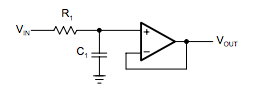
\includegraphics[width=\textwidth]{figures/cProblemloesning/Lavpasfilter1_teoretisk.PNG}
		\caption{På figuren ses en illustration af et 1. ordens unity-gain Sallen-Key lavpasfilter, hvor værdien C er kondensatoren, R er modstandene. filterKonfigurationen har en indgangsspænding, Vin og udgangsspænding, Vout. \citep{Carter2013}}
		\label{fig:SallenKey1}
	\end{minipage}
	\hfill
	\begin{minipage}[b]{0.45\textwidth}
		\includegraphics[width=\textwidth]{figures/cProblemloesning/Sallenlavpas.PNG}
		\caption{På figuren ses en illustration af et 2. ordens unity-gain Sallen-Key lavpasfilter, hvor værdien C er kondensatoren, R er modstandene. filterKonfigurationen har en indgangsspændings, Vin og en udgangsspænding, Vout. \citep{Carter2013}}
		\label{fig:SallenKey2}
	\end{minipage}
\end{figure}

I designet af et 3. ordens filter designes, som sagt, både et 1. og et 2. ordens filter i forlængelse af hinanden. Dette designes efter sallen-key metoden bestående af tre modstande, tre kondensatorer og to operationsforstærkere. Værdierne for modstandene kan udregnes ved \eqref{eq:Lavpas1Modstande} for et 1. orden lavpasfilter og \eqref{eq:LavpasModstande} for et  2. orden lavpasfilter.  
\begin{equation} \label{eq:Lavpas1Modstande}
R_{1} = \frac{a_1}{2 \cdot \pi \cdot f_c \cdot C_1} \\
\end{equation}
\begin{equation}
 \label{eq:LavpasModstande}
R_{1,2} = \frac{a_1 \cdot C_2 \pm \sqrt{A_1^2 \cdot C_2^2 - 4 \cdot b_1 \cdot C_1 \cdot C_2}}{4 \pi \cdot f_c \cdot C_1 \cdot C_2}
\end{equation}

\noindent Værdierne for $a_{1}$ og $b_{1}$ findes i en tabel, hvor konstanterne for et butterworthfilter fremgår. Af denne grund findes værdien for $a_{1}$  og  $b_{2}$, der begge er 1.0000. For at finde reelle værdier under kvadratroden skal følgende være opfyldt:
\begin{equation} \label{eq:kondensator}
C_2 \geq C_1 \frac{4b_1}{a_1^2}
\end{equation}
I ovenstående \eqref{eq:LavpasModstande} er C variabler for kondensatorer, R er variabler for modstande og $a_1$ og $b_1$ er konstanter, mens $f_c$ er den valgte knækfrekvens, jævnfør kravspecifikationerne afsnit \ref{FilterAfs} på side \pageref{FilterAfs}. 

\noindent For at udregne modstandene fastsættes $C_1$ til 100nF for hhv. både 1. og 2. ordens lavpasfiltrene. Når $C_1$ er bestemt, kan $C_2$ for 2. ordens lavpasfilteret beregnes ved at benytte følgende \eqref{eq:kondensator}. Som grundregel skal $C_2$ være over dobbelt så stor som $C_1$:
\begin{equation}  
C_2 \geq 100\text{nF} \frac{4\cdot 1}{1.000^2} = C_2 \geq 200\text{nF}
\end{equation}

\noindent Ud fra ovenstående ligning vælges $C_2$ til at være 480nF for at opfylde \eqref{eq:kondensator}. Når værdierne for C er bestemt kan modstandene for filteret bestemmes. For et 1. orden lavpasfilter benyttes \eqref{eq:Lavpas1Modstande} til at beregne $R_1$ og for et 2. ordens lavpasfilter anvendes \eqref{LavpasModstande} for at beregne $R_1$ og $R_2$. 
\begin{equation} \label{eq:1ordenmodstand}
R_{1} = \frac{1}{2 \cdot \pi \cdot 25 \cdot 100nF} R_{1} = 63661.98 \Omega
\end{equation}
\begin{equation} \label{eq:2ordenmodstand}
R_{1,2} = \frac{1.0000 \cdot 480\text{nF} \pm \sqrt{1.0000^2 \cdot 480\text{nF}^2 - 4 \cdot 1.0000 \cdot 100\text{nF} \cdot 480\text{nF}}}{4 \pi \cdot 25\text{Hz} \cdot 100\text{nF} \cdot 480\text{nF}} = \begin{cases} R_{1} =  44825.94\Omega \\ R_{2} = 18836.04 \Omega \end{cases}
\end{equation}
\noindent Filterets værdier for kondensatoerne og modstandene er nu udregnet for hhv. 1. og 2. ordens filter. Filterkonfigurationen kan nu simuleres i LTspice for at bestemme, hvor godt et 3. ordens filter, der er blevet designet.

\begin{figure}[H]
	\centering
	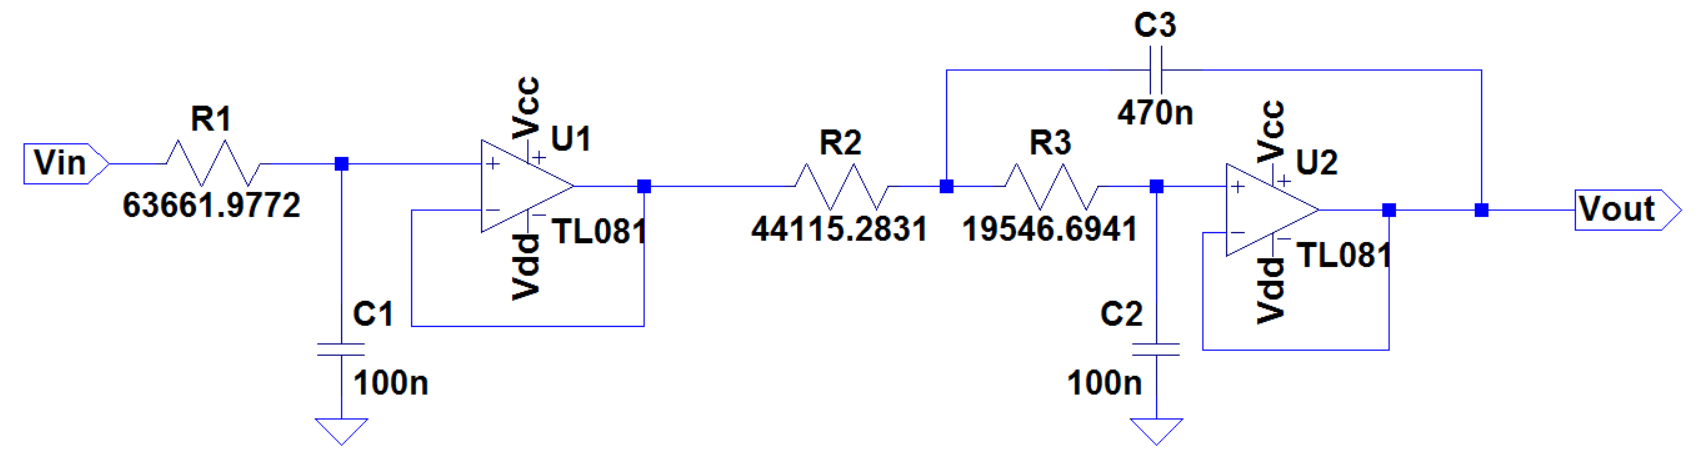
\includegraphics[scale=0.5]{figures/cProblemloesning/Lavpasfilter1_LTspice.PNG}
	\caption{Af figuren fremgår det teoretiske kredsløb for lavpasfilteret med udregnede værdier for de enkelte modstande og kondenstatorer. På figuren fremgår værdierne $R_{2}$ og $R_{3}$, hvilket svarer til de udregnede værdier $R_{1}$ og $R_{2}$ for 2. ordens filteret i \eqref{eq:2ordenmodstand}. Filteret er designet i LTspice.}
	\label{fig:lavpasfilter1_LTspice}
\end{figure}

\subsubsection{Simulering}
For at udføre en simulering af 3. ordens lavpasfilteret, foretages en AC-analyse, der beskriver forholdet mellem frekvensindholdet og filterets dæmpning. Kredsløbet simuleres med et inputsignal, der har en amplitude på $1$V. Jævnfør kravspecifikationerne afsnit \ref{FilterAfs}, side \pageref{FilterAfs} er knækfrekvensen bestemt til at være $25$Hz og stopbåndsfrekvensen til $45$Hz grundet resultater fra pilotforsøget i afsnit \ref{sec:pilotforsoeg}, side \pageref{sec:pilotforsoeg}. LTspice anvendes til simulering af lavpasfilteret, hvor der anvendes operationsforstærkeren, TL081, hvilket er den operationsforstærker, der også vil blive benyttet i test af filteret. I simuleringen vil der blive undersøgt, hvorledes kravene stemmer overens med kravspicifikationerne, ved at betragte et bodeplot over det simulerede 3. ordens filter.

\begin{figure}[H]
	\centering
	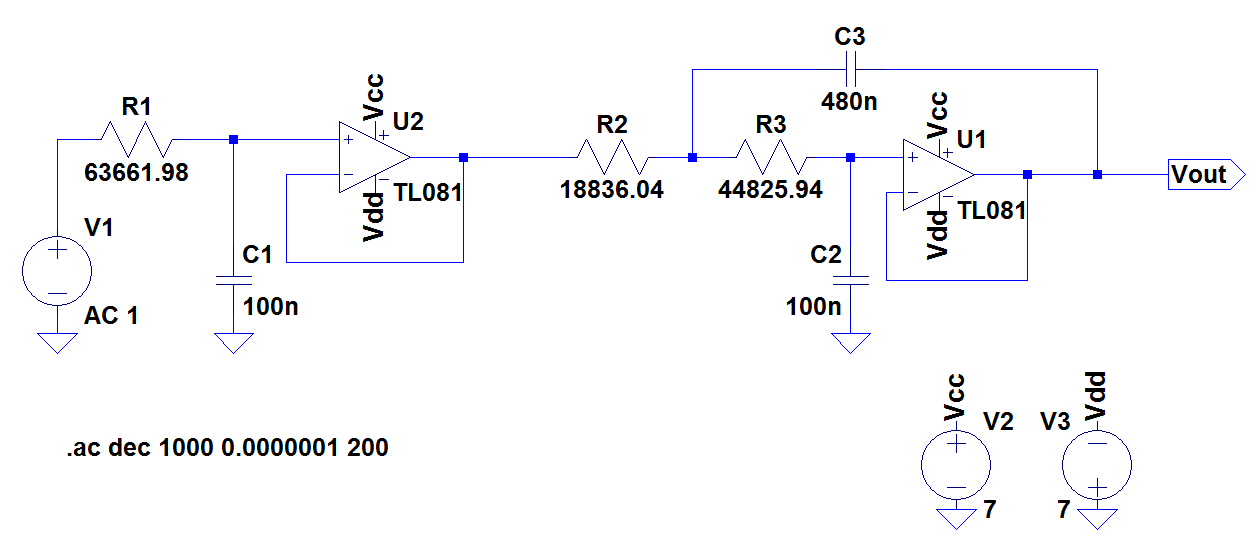
\includegraphics[scale=0.45]{figures/cProblemloesning/Lavpasfilter_LTspice.PNG}
	\caption{Af figuren fremgår en illustration af kredsløbet for et 3. ordens lavpasfilter. Filteret simuleres i LTspice vha. en AC-analyse med et inputsignal, der har en amplitude på $1$V.}
	\label{fig:lavpasfilter_LTspice}
\end{figure}

\begin{figure}[H]
	\centering
	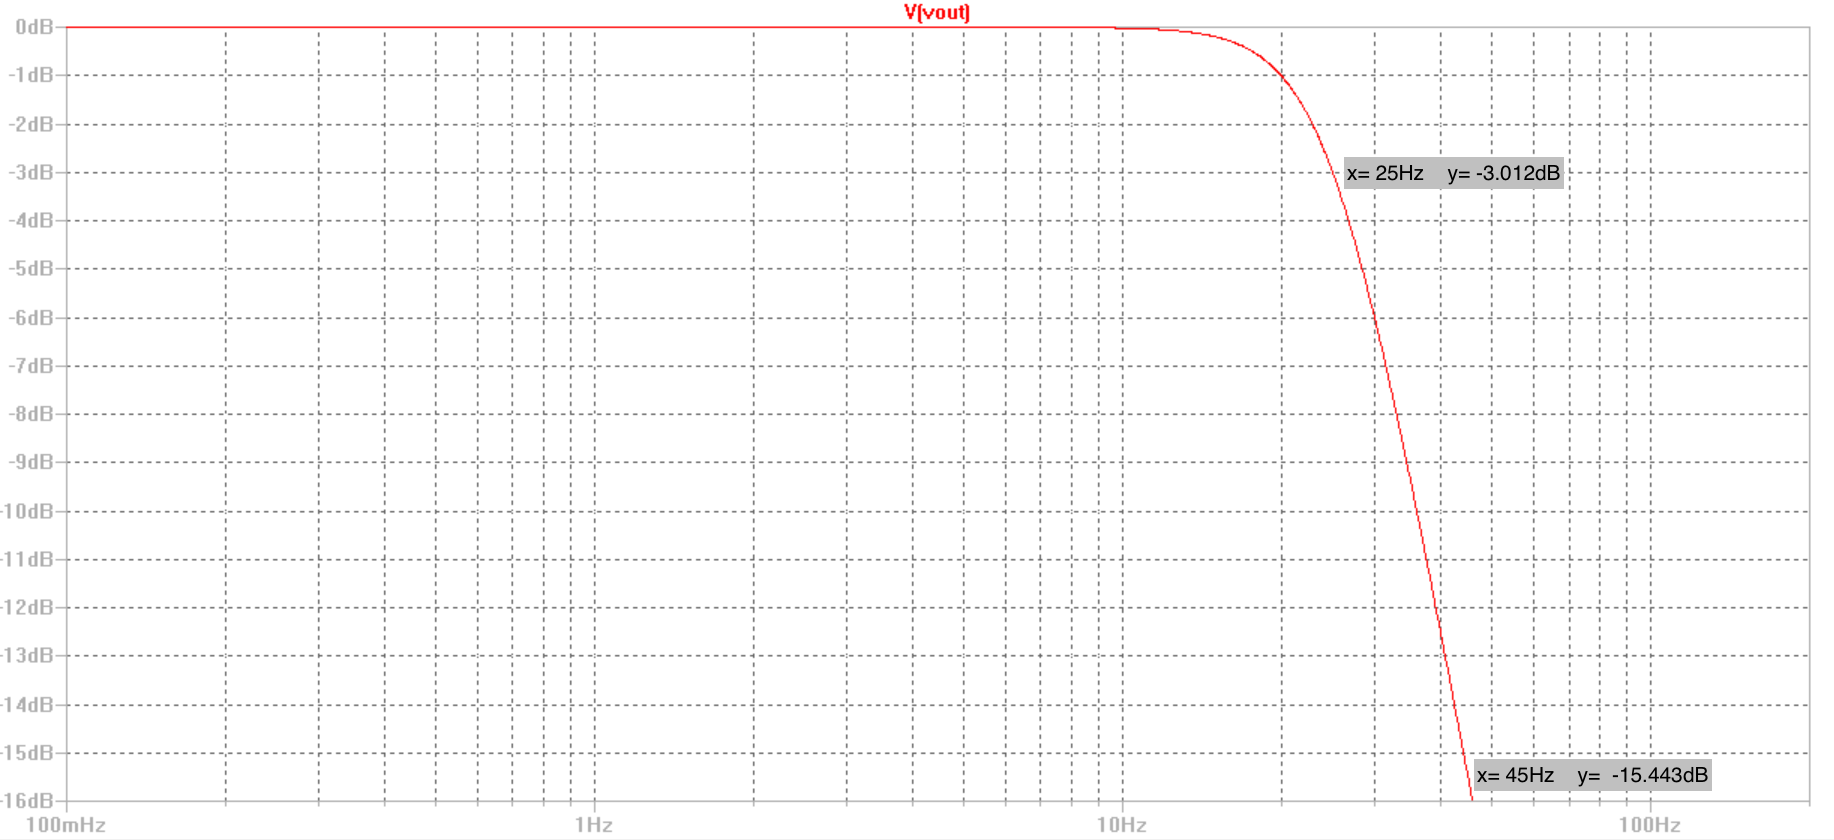
\includegraphics[scale=0.4]{figures/cProblemloesning/Lavpasfiltergraf_LTspice1.PNG}
	\caption{Af figuren fremgår en illustration på et bodeplot, der viser 3. ordens filterets frekvensindhold målt i Hz over dæmpningen målt i dB. Lavpasfilteret er simuleret i LTspice.}
	\label{fig:lavpasfilter_LTspice}
\end{figure}

Af bodeplottet fremgår det, at det simulerede filter har en maksimal amplitude i db på XX \fxnote{skla være under 3 db} ved en knækfrekvens på $25$Hz, hvilket overholder kravspecifikationerne i afsnit \ref{FilterAfs}, side \pageref{FilterAfs}. Der aflæses, at der ved stopbåndsfrekvens på $45$Hz er en amplitude i db på $15.49$. Dette overholder projektets opstillede krav for filterkonfigurationen ved en minimum dæmpning på $14$ dB i stopbåndsfrekvensen.  


\subsubsection{Implementering og test} 
Der ses på \figref{fig:lavpasfilter_LTspice} at der benyttes 3 modstande og 3 kondensatorer til at designe kredsløbet. Reelt findes de udregnede modstande og kondensatorer ikke, og derfor benyttes der dem som kommer tættest på det teoretiske. Dette gøres ved at sætte både modstande og kondensatorer i henholdsvis serie- og parallelforbindelse for at opnå de ønskede værdier. For $R_{1}$ og $R_{2}$ anvendes der modstande i parallelforbindelse og for $R_{3}$ i serieforbindelse. For $C_3$ anvendes der kondensatorer i parallelforbindelse. Der foretages målinger på tre ens reelle modstande og kondensatorer for at kunne anvende de komponenter som afviger mindst fra de teoretiske værdier. Dette er illustreret i \tableref{Tab:Maalingfilter}
\begin{table}[H]
	\centering
	\begin{tabular}{|l|l|l|l|}
		\hline
		\textit{}                                     & \textit{Teoretisk} & \textit{Måling}    & \textit{Afvigelse} \\ \hline
		\multirow{2}{*}{\textit{$R_{1}$(Parallel) :}} & $1$M$\Omega$       & $1.0046$M$\Omega$  & $0.46\%$           \\ \cline{2-4} 
		& $68$K$\Omega$      & $68.0350$K$\Omega$ & $0.05\%$           \\ \hline
		\multirow{2}{*}{\textit{$R_{2}$(Parallel) :}} & $1$M$\Omega$       & $1.0037$K$\Omega$  & $0.37\%$           \\ \cline{2-4} 
		& $47$K$\Omega$      & $47.0540$K$\Omega$ & $0.11\%$           \\ \hline
		\multirow{2}{*}{\textit{$R_{3}$(Serie) :}}    & $18$K$\Omega$      & $17.9600\Omega$    & $0.22\%$           \\ \cline{2-4} 
		& $820\Omega$        & $816\Omega$        & $0.49\%$           \\ \hline
		\textit{$C_{1}$ :}                            & $100$n             & $98$n              & $2.00\%$           \\ \hline
		\multirow{2}{*}{\textit{$C_{2}$(Parallel) :}} & $470$n             & $464$n             & $1.29\%$           \\ \cline{2-4} 
		& $10$n              & $9$n               & $10\%$             \\ \hline
		\textit{$C_{3}$ :}                            & $100$n             & $98$n              & $2.00\%$           \\ \hline
	\end{tabular}
	\caption{I tabellen ses der, at de anvendte modstande og kondensatorer afviger fra den teoretiske værdi, hvilket er forventet af reelle komponenter. Det er en acceptabel afvigelse, så modstandene kan derfor anvendes til implementering}
	\label{Tab:Maalingfilter}
\end{table}
Herefter implementeres kredsløbet. I testen anvendes en spændingsforsyning på $5.5$V og en funktionsgenerator som inputsignal, samt et multimeter til aflæsning af dæmpningen. Funktionsgeneratoren sættes til de ønskede frekvenser i intervaller af $1$Hz fra $10$Hz til $50$Hz. Outputtet i dB måles for hver frekvens. Ud fra disse målinger plottes en graf af dæmpningen i MatLab, hvilket er illustreret på \figref{fig:Lavpas_Matlab}.  

\begin{figure}[H]
	\centering
	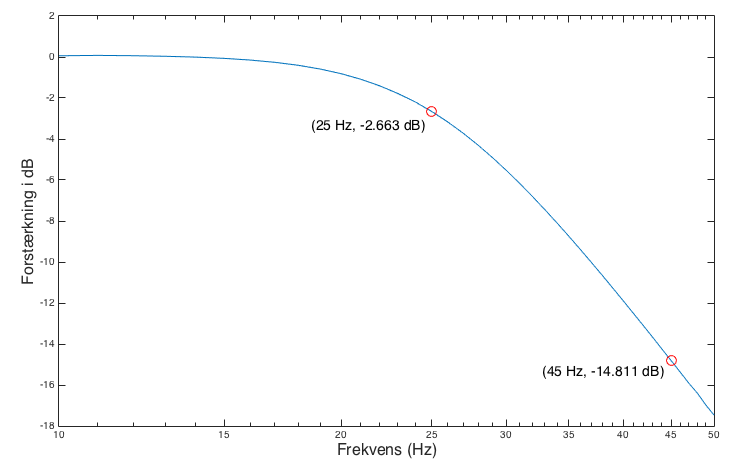
\includegraphics[scale=0.4]{figures/cProblemloesning/Lavpas_Matlab.PNG}
	\caption{Figuren viser dæmpningen som en graf over de målte frekvenser i Hz som funktion af outputtet i dB. På grafen er der angivet knækfrekvens og stopbåndfrekvens}
	\label{fig:Lavpas_Matlab}
\end{figure}

%Sammenlignes værdierne fra \ref{Lavpas_Matlab} for det testede kredsløb med værdierne fra \ref{fig:lavpasfilter_LTspice} for det simulerede kredsløb ses der en ændring i frekvens og dæmpning, hvilket også er forventet grundet andre kodensatorer og modstande. 

%\begin{table}[H]
%	\centering
%	\begin{tabular}{|l|l|l|l|}
%		\hline
 %  & \textit{Simulering} 	& \textit{Test}  &\textit{Afvigelse} \\ \hline
%Knækfrekvens	 & $25Hz$ 			& $25.0308Hz$			& $4\%$  \\ %\hline
%Stopbåndsfrekvens & $45Hz$		& $45.0816Hz$			& $0.18\%$ \\ \hline
%Dæmpning på stopbånd & $15.489dB$  & $14.881dB$     & $9.61\%$  \\ \hline
%Dæmpning på pasbånd & $3.0273dB$	  & $2.663dB$  & $13.68\%$  \\ \hline
%	\end{tabular}
%	\caption{I tabellen ses afvigelserne for hhv. knækfrekvens, stopbåndsfrekvens og dæmpning af stopbånd og pasbånd ift. simlering og test}
%	\label{Tab:Afvigelse_simulering}
%\end{table}

Ud fra de testede værdier i \tableref{Tab:Tolerance} og kravspecifikationer i afsnit \ref{filterAfs} på side \pageref{filterAfs} er der er ingen afvigelse på knækfrekvensen og stopbåndsfrekvensen. Der er en variation ift. dæmpningen for både stop- og pasbånd på hhv. $6.36\%$ og $8.37$\% i forhold til kravet.

\begin{table}[H]
	\centering
	\begin{tabular}{|l|l|l|l|}
		\hline
   & \textit{Krav} 	& \textit{Test}  &\textit{Afvigelse} \\ \hline
Knækfrekvens	 & $25Hz$ 			& $25Hz$			& $0\%$  \\ \hline
Stopbåndsfrekvens & $45Hz$		& $45Hz$			& $0\%$ \\ \hline
Dæmpning på stopbånd & $14dB$    & $14.8910dB$    & $6.36\%$  \\ \hline
Dæmpning på pasbånd & $3dB$		& $2.7490dB$	    & $8.37\%$ \\ \hline
	\end{tabular}
	\caption{I tabellen ses afvigelserne for hhv. knækfrekvens, stopbåndsfrekvens og dæmpning af stopbånd og pasbånd ift. krav og test}
	\label{Tab:Tolerance}
\end{table}
\noindent I forhold til tolerancekravene i afsnit \ref{FilterAfs} på side \pageref{FilterAfs} skulle dæmpningen på stopbåndet være minimum $14 dB$ og måtte maksimalt have en afvigelse herfra på $+10\%$. Denne tolerance overholdes ved testen, da de acceptable dæmpningsværdier vil ligge i intervallet $14$-$15.4$db. For pasbåndet skulle dæmpningen maksimalt være $3$dB med en maksimal afvigelse på $-15\%$. Dette vil sige at testen passer inden for tolerancekravene, da der accepteres værdier i intervallet $2.55$-$3$dB. På baggrund af dette accepteres alle målte afvigelser ved testen af filteret.